\documentclass[tikz]{standalone}
%\usepackage[dvipsnames]{xcolor}
\usepackage{amsmath}
\usepackage{amssymb}
\usepackage{setspace}
\usepackage{xeCJK}
\usepackage{ulem}
\usepackage{pstricks}
\usepackage{pstricks-add}
\usepackage{bm}
\usepackage{mathtools}
\usepackage{breqn}
\usepackage{mathrsfs}
\usepackage{esint}
\usepackage{textcomp}
\usepackage{upgreek}
\usepackage{pifont}
\usepackage{tikz}
\usepackage{circuitikz}
\usepackage{caption}
\usepackage{tabularx}
\usepackage{array}
\usepackage{pgfplots}
\usepackage{multirow}
\usepackage{pgfplotstable}
\usepackage{mhchem}

\setCJKfamilyfont{boldsong}[AutoFakeBold = {2.17}]{SimSun}
\newcommand*{\boldsong}{\CJKfamily{boldsong}}
%\DeclareMathOperator\dif{d\!}
\newcommand*{\me}{\mathop{}\!\mathrm{e}}
\newcommand*{\mpar}{\mathop{}\!\partial}
\newcommand*{\dif}{\mathop{}\!\mathrm{d}}
\newcommand*{\tab}{\indent}
\newcommand*{\mcelsius}{\mathop{}\!{^\circ}\mathrm{C}}
\renewcommand*{\Im}{\mathrm{Im}\,}

\begin{document}
	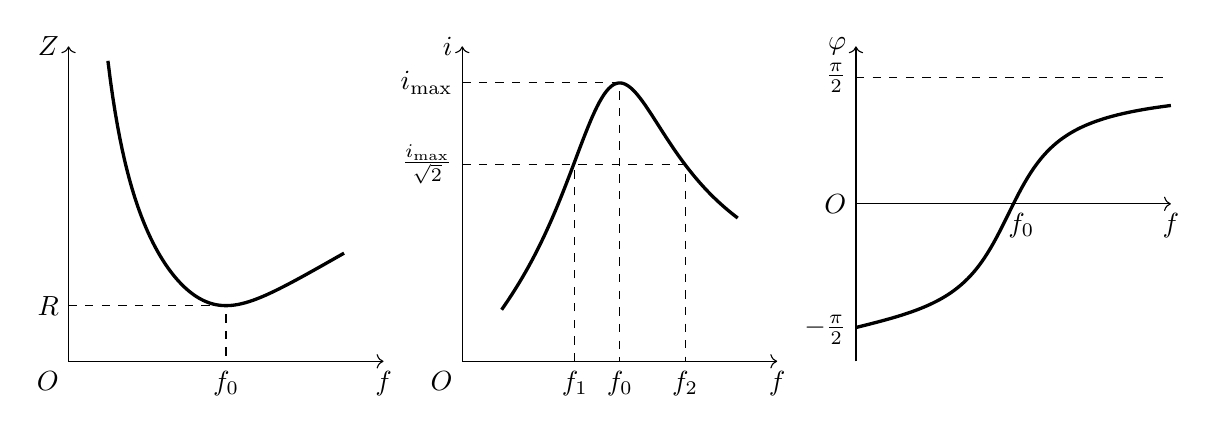
\begin{tikzpicture}
		\draw[<->] (0,4)node[left]{$ Z $}--(0,0)node[below left]{$ O $}--(4,0)node[below]{$ f $};
		\draw[very thick,domain=0.5:3.5,samples=100] plot (\x,{sqrt(0.5+pow(0.5*\x-1/\x/0.5,2))});
		\draw[dashed] (0,0.707)node[left]{$ R $}--(2,0.707)--(2,0)node[below]{$ f_0 $};
		
		\draw[<->] (5,4)node[left]{$ i $}--(5,0)node[below left]{$ O $}--(9,0)node[below]{$ f $};
		\draw[very thick,domain=5.5:8.5,samples=100] plot (\x,{2.5/sqrt(0.5+pow(0.5*(\x-5)-1/(\x-5)/0.5,2))});
		\draw[dashed] (5,3.536)node[left]{$ i_\max $}--(7,3.536)--(7,0)node[below]{$ f_0 $};
		\draw[dashed] (5,2.5)node[left]{$ \frac{i_\max}{\sqrt 2} $}--(7.83,2.5)--(7.83,0)node[below]{$ f_2 $};
		\draw[dashed] (6.43,0)node[below]{$ f_1 $}--(6.43,2.5);
		
		\draw[->] (10,0)--node[left,midway]{$ O $}(10,4)node[left]{$ \varphi $};
		\draw[->] (10,2)--(14,2)node[below]{$ f $};
		\draw[,very thick,domain=10.01:14,samples=100] plot (\x,{2+rad(atan((\x-10)*0.5*2-1/(\x-10)/0.25))});
		\node[left] at(10,0.4) {$ -\frac\pi 2 $};
		\draw[dashed] (10,3.6)node[left]{$ \frac\pi2 $}--(14,3.6);
		\node[below] at(12.1,2) {$ f_0 $};
	\end{tikzpicture}
\end{document}